
%(BEGIN_QUESTION)
% Copyright 2009, Tony R. Kuphaldt, released under the Creative Commons Attribution License (v 1.0)
% This means you may do almost anything with this work of mine, so long as you give me proper credit

Build a simple circuit using either a light sensor (photocell) or a temperature sensor (thermistor) connected to a fixed-value resistor and a battery such that a variable output voltage will be generated as the sensor is stimulated.  Your circuit must either make the voltmeter indication increase with increasing sensor stimulus (more voltage for more light or heat -- direct action), or do the exact opposite (reverse action), as specified by the instructor.  All electrical connections must be made using a terminal strip (no twisted wires, crimp splices, wire nuts, spring clips, or ``alligator'' clips permitted).  You will also need to demonstrate how to record and display the lowest and highest voltages output by this circuit using your digital multimeter's ``min/max'' recording function function.

This exercise tests your ability to properly identify the operating characteristics of a light or temperature sensor, properly size a resistor to form a voltage divider circuit with the sensor, properly connect a voltmeter into the circuit to achieve the specified response direction, properly use a DMM to capture minimum and maximum voltage values, and use a terminal strip to organize all electrical connections.

$$\includegraphics[width=15.5cm]{i03776x01.eps}$$

\vskip 10pt

The following components and materials will be available to you during the exam: assorted CdS {\bf photocells} and {\bf thermistors} ; an assortment of {\bf resistors} ; {\bf terminal strips} ; lengths of {\bf hook-up wire} ; {\bf battery clips} (holders).

\vskip 10pt

You will be expected to supply your own screwdrivers and digital multimeter (DMM) for assembling and testing the circuit at your desk.  The instructor will supply the battery(ies) to power your circuit when you are ready to see if it works.  Until that time, your circuit will remain unpowered.

\vskip 10pt

\noindent
{\bf Meter response} (instructor chooses): \hskip 20pt \underbar{\hskip 20pt} Direct \hskip 20pt \underbar{\hskip 20pt} Reverse

\vskip 10pt

\noindent
{\bf Captured value} (instructor chooses): \hskip 20pt \underbar{\hskip 20pt} $V_{minimum}$ \hskip 20pt \underbar{\hskip 20pt} $V_{maximum}$

\vskip 10pt

\noindent
{\bf Sensor type} (instructor chooses): \hskip 20pt \underbar{\hskip 20pt} Photocell \hskip 20pt \underbar{\hskip 20pt} Thermistor

\vfil

%Study reference: the ``Analog Electronic Instrumentation'' chapter of {\it Lessons In Industrial Instrumentation}.

\underbar{file i03776}
%(END_QUESTION)





%(BEGIN_ANSWER)


%(END_ANSWER)





%(BEGIN_NOTES)


%INDEX% Mastery exam performance exercise (circuit), light/temp voltage divider circuit

%(END_NOTES)


